\section{Part 2}
\subsection{How to design LQI controller}

A stationary LQR can be used to find the feedback control gain K, which minimizes thefollowing quadratic cost, with respect to a control input u(t):

\begin{equation}
    \begin{aligned}
        J=\dfrac{1}{2}\int_0^\infty\left(x(t)^TQ_xx(t)+u(t)^TQ_uu(t)\right)dt
    \end{aligned}
\end{equation}

where $ Q_x $ and $ Q_u $ are weighting matrices, telling the controller about  the priorities of tunning states and control signals.

The original LQR method can be extended to achieve reference tracking. To do this, the system needs to be augmented with integral states $z_i$, which allow the computation of the cumulative tracking error $ \int (y-r)dt $ :
\begin{equation}
    \begin{aligned}
        \begin{bmatrix}
             \dot{x}(t)\\\dot{z}(t)\end{bmatrix}=\underbrace{\begin{bmatrix}A_\delta&0\\C_I&0\end{bmatrix}}_{A_{aug}}\begin{bmatrix}x(t)\\z(t)\end{bmatrix}+\underbrace{\begin{bmatrix}B_\delta\\0\end{bmatrix}}_{B_{aug}}u(t)+\begin{bmatrix}K_r\\-I\end{bmatrix}r(t)
    \end{aligned}
\end{equation}

\begin{equation}
    \begin{aligned}
        u(t)=-K\begin{bmatrix}x(t)\\z(t)\end{bmatrix}=-[K_PK_I]\begin{bmatrix}x(t)\\z(t)\end{bmatrix}
    \end{aligned}
\end{equation}

where $C_I$ selects the system states needed to compute the new integral states, and $ K $ can be calculated by Matlab function \texttt{lqr}.

\subsection{Application and verify}

For the assignment 1 part 2, the system does not have other input singals expect a singal reference signal $ \mathbf{r} $.

The augmented system is :
\begin{equation}
    \begin{aligned}
        &\begin{bmatrix}\dot{x}\\\dot{x}_i\end{bmatrix}=\begin{bmatrix}A&0\\-C&0\end{bmatrix}\begin{bmatrix}x\\x_i\end{bmatrix}+\begin{bmatrix}B\\0\end{bmatrix}u+\begin{bmatrix}0\\0\\0\\0\\1\end{bmatrix}r\\
        &\mathbf{A_{aug}} = \begin{bmatrix}A&0\\-C&0\end{bmatrix} \\
        &\mathbf{B_{aug}} = \begin{bmatrix}0\\0\\0\\0\\1\end{bmatrix}
    \end{aligned}
\end{equation}

where $ \mathbf{C} $ is selected as $ \mathbf{C(1,:)} $, since $\mathbf{y = Cx }$ and $ y_1=\alpha $.

Select $Q,  R$ after tunning:

\begin{lstlisting}
    Q = diag([0 100 0 0 0 1]);
    R = diag([1 1 1]);       
\end{lstlisting}

And use the build- in function to get the $ K $ matrix:

\begin{lstlisting}
    [K,~ ,~] = lqr(A_aug, B_aug, Q, R)
\end{lstlisting}

Now rebuild the new closed loop feedback system as :

\begin{lstlisting}
    Ae = [A_lqr-B_lqr*K]; % 6x6
    Be = [0 0 0 0 0 1]'; % 6x1
    Ce = [C zeros(3, 1)]; % 3x6
    De = 0; % 1x1
    sys_e = ss(Ae, Be, Ce, De);
\end{lstlisting}

The respond of a step signal shows below:

\begin{figure}[H]
 \centering
 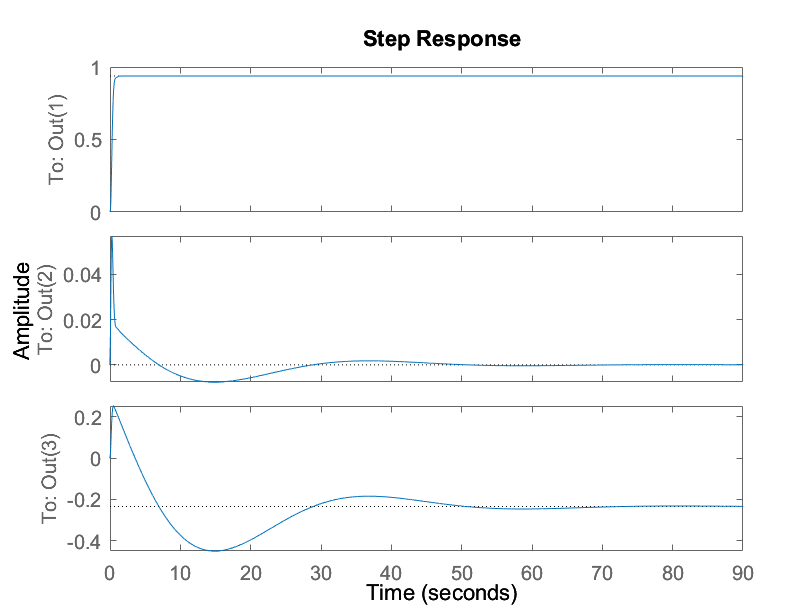
\includegraphics[width=0.8\textwidth]{images/step.png}
 \caption{Step respond}
 \label{step}
\end{figure}

From the picture \ref{step}, it is clear we achieved a reference tracking for the state $ \alpha $.

  
